\section{Principles of Manifestation}


\begin{wrapfigure}{rt}{0.35\textwidth}
\centering
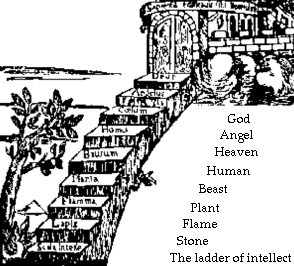
\includegraphics[scale=.5]{a20141119PrinciplesofManifestation-img001.png} 
\caption{Great Chain of Being}
\end{wrapfigure}
 
If cosmology is the study of the origin, nature, and destiny of the universe, there have been many conflicting theories. In the West, the basis of cosmology has been what is called the \textbf{Great Chain of Being}. In various versions, it has formed the worldview of educated people until recently. The dominance of profane science has done much to discredit it, even to the point that exoteric spiritual teachings not only neglect it, but in effect oppose it. This often has less to do with science than with ideology.

The Great Chain of Being is based on certain Traditional metaphysical principles. These need to be made clear, but first the implicit principles of modernity must be made clear.

\paragraph{Profane Worldview}
In its most consistent form, the modern worldview is based on the notion that the origin, nature, and destiny of the universe can be fully explained in terms of matter and energy. Obviously, this worldview denies that there is a world of Being ontologically prior to, and superior to, the world of Becoming. Profane science needs to explain:

\begin{enumerate}
\item How emergent properties such as life, mind, consciousness, emotions, thought, in short, interiority, evolve from material and exterior processes. 
\item How higher order systems are constructed from more basic elements. 
\end{enumerate}
Thus far, science has no answer to issue (1), not even a plausible theory. Issue (2) is often hidden in popular discourse. Profane science is committed to reductionism, viz., higher order systems are fully explicable by more fundamental elements. By denying the existence of essences or forms, the task of science is to define higher systems; in its most consistent philosophical expressions, these are mere “social constructs”.

\paragraph{Evolution and Involution}
\textbf{Rene Guenon} explains that there are five conditions of manifestation: space, time, form (or essences), matter, and life. The opposite of “evolution” is not creation science, or even intelligent design, but rather involution.

Evolution is the notion that simple things evolve into complex structures caused by random variations over time. Involution is the notion that ideal essences are brought into manifestation by a will. Depending on the strength of the will, the existing being will be a better or worse copy of its ideal.

Essences unfold in space and time, thus appearing to be evolving (e-volve = unfold), but really involving. For example, Beethoven's Ninth Symphony is an “idea” or essence. However, to be experienced, musicians and instruments are necessary for the symphony to unfold in time. Profane science has nothing to offer. It makes no sense to say that the first movement “causes” the final movement. A fortiori, it is risible to try to experience or understand the symphony from an analysis of its individual notes.

Hence, Guenon claims that the higher order system defines its components, rather than the other way around. The other point is that “life” is prior to matter. So, in a sense, everything is “alive”, that is, it has interiority. Hence, esoterism understands the cosmos as an interior process, unlike an astronomer who takes the opposite approach.

\paragraph{The Idea of the Good}
Plato understood God to be the Idea of the Good. Hence, man's goal is to passively contemplate the Good. The Christian notion of God as Love builds on that, since Love means to will the good. It is a revealed truth that the created world is “good”, so the good is whatever has more being. The goodness of God, then, is His creative activity. So to be godlike is also to be creative, in the sense of bringing essences into manifestation. The gap between the essence and its existence is privation, i.e., “evil”.

\paragraph{Rationality and Intellectuality}
Rationality is the quality that distinguishes man from animals; intellectuality distinguishes God from man. Rationality involves dualist thinking, but intellectuality is non-dual. It is not irrational, but rather super-rational. Any attempt to conceive of God's knowledge and will in rational terms will fail. For example, I read on a web site a few months back the claim that “God knows all true propositions.” Not at all, God knows the Divine ideas directly and non-dually, not as propositions. He “knows” the world because He created it. There is not duality of essence and existence for God.

Similarly for the Divine Will, there is no distinction between freedom and necessity. God does not “deliberate”, choosing this or that, but rather whatever exists is the expression of his Goodness. Some will claim that God cannot do things like creating a square circle. It is better to understand that as a possibility of non-manifestation. There are four such possibilities.

\begin{enumerate}
\item \textbf{Analytic}. The definition contains a self-contradiction (as in the example above). 
\item \textbf{Synthetic}. The contradiction is not in the definition. “A colored thing must also be extended.” 
\item \textbf{Physical}. The human frame has an upper limit, since as an increase in height is linear, the increase in mass is cubic. Hence, the skeletal structure will not be able to support that weight. 
\item \textbf{Compossibility}. Certain possibilities of manifestation cannot manifest in the same place or time 
\end{enumerate}
The loss of intellectuality in the modern world has consequences. First of all, rationality tries to take its place; it is doomed to failure. The next step is that emotionality, i.e., the subrational, as a sort of non-dual experience, usurps the place of true non-dual intellectuality. Hence, Love is understood not as the creative Will to being, but rather in a sentimental and humanitarian way as compassion and the alleviation of suffering.

The modern mind misunderstands evil and thinks there is a “problem of evil” to be explained. However, the teaching is that creation is good, so that the world of good and evil that we experience is the creation of man. If the cheetah chases the gazelle, the result is good for the cheetah since it increase his being, but bad for the gazelle since his being is ended; however, there is no question of “evil” in that scenario. On the contrary, it is good that the gazelle was given being in the first place.

\paragraph{Principle of Plenitude}
In the \emph{Multiple States of Being}, Rene Guenon showed that the Absolute must also be Infinite, that is, the number of possibilities is unbounded. He formulated the Principle of Plenitude as “All possibilities of manifestation must be manifested.”

This accounts for the immense variety in the world. Every creature has its place in the chain, or scale, of being. It is irrational to expect everything to be the same, so the scale is hierarchically arranged. Moreover, there are many more scales of being than the one that describes our world.

\paragraph{Principle of Continuity}
A related principle is the Principle of Continuity, described in the \emph{Metaphysical Principles of Infinitesimal Calculus}. The gaps in the scale become arbitrarily small. Thus, we see that a taxonomic problem arises in biology, since it can become difficult to distinguish between closely related species and subspecies. Hence, there is no absolute definition of a species. That problem is insoluble as long as biological and material considerations are the only criteria used. In such a case, definitions are considered arbitrary social constructs.

Of course, the Traditional view is different. These close differences nevertheless reflect different essences in the Divine mind. Proper classifications will have to take the soul and spiritual elements (i.e., “interiority”) into account. Hence, the differences are real, no matter how close they may appear. There are some further points that can be derived from this principle, although they cannot be fully developed in this post:

\begin{itemize}
\item The attempt to refute Darwinian evolution by pointing to “missing links” in the fossil record (yes, the term is derived from the Great Chain of Being) is actually anti-Traditional. 
\item The Great Chain of Being is a simplification. It is better represented as scales within scales. 
\item \textbf{Otto Weininger} in \emph{Sex and Character} defines the ideal masculine and feminine qualities. However, they don't manifest in a strictly binary way, but rather on a scale ranging from absolute femininity to absolute masculinity. 
\item Intellectual movements always ramify into two competing camps whenever the possibility of a dispute arises. For example, a predestinarian Baptist church will give rise to a “free-will Baptist church”. In other cases, movements will split by incorporating elements from other, often incompatible, movements. This is why all movements are prone to degeneration and inner conflict. 
\end{itemize}
\flrightit{Posted on 2014-11-19 by Cologero }

\begin{center}* * *\end{center}

\begin{footnotesize}\begin{sffamily}



\texttt{Constantine on 2014-11-19 at 14:25 said: }

Reading through this article I felt something was missing. You make a good point fractal, what about energy (chi, prana…)?


\hfill

\texttt{Francesco on 2014-11-19 at 16:14 said: }

Constantine: Imo, Qi can be handled under the five conditions of manifestation, some more than others Perhaps in the same way that Sophia is not a fourth hypostasism but the life shared in common by the trinity; Qi is not another condition, but something shared commonly among form, matter, and life. 

In Chinese metaphysics, there are a great number of “Qis”: human body qi (then specific organ and system qi types), cosmological qi (astrology), environmental qi (feng shui), and so on. To see how better how this concept is subsumed in the five conditions, we might consider the famous Chinese character for Qi–which is a pot of rice gruel cooking, with steam raising from the vessel lid–it is interpreted as “it moves”, or “acts”.

The Classics explain “Qi is the commander of Blood; Blood is the mother of Qi”, and that “Qi follows where the Shen (consciousness) leads”.


\hfill

\texttt{Cologero on 2014-11-19 at 17:37 said: }

@Constantine: “Matter is condensed energy and energy is condensed consciousness.” \flright{\textsc{Valentin Tomberg}}


\end{sffamily}\end{footnotesize}
